\begin{frame}
    \frametitle{Measurement}
    \small
    A high density accelerometer is used to monitor the roller bearing.  The accelerometer can be either permanently mounted or a portable device.
    \begin{figure}
        \centering
        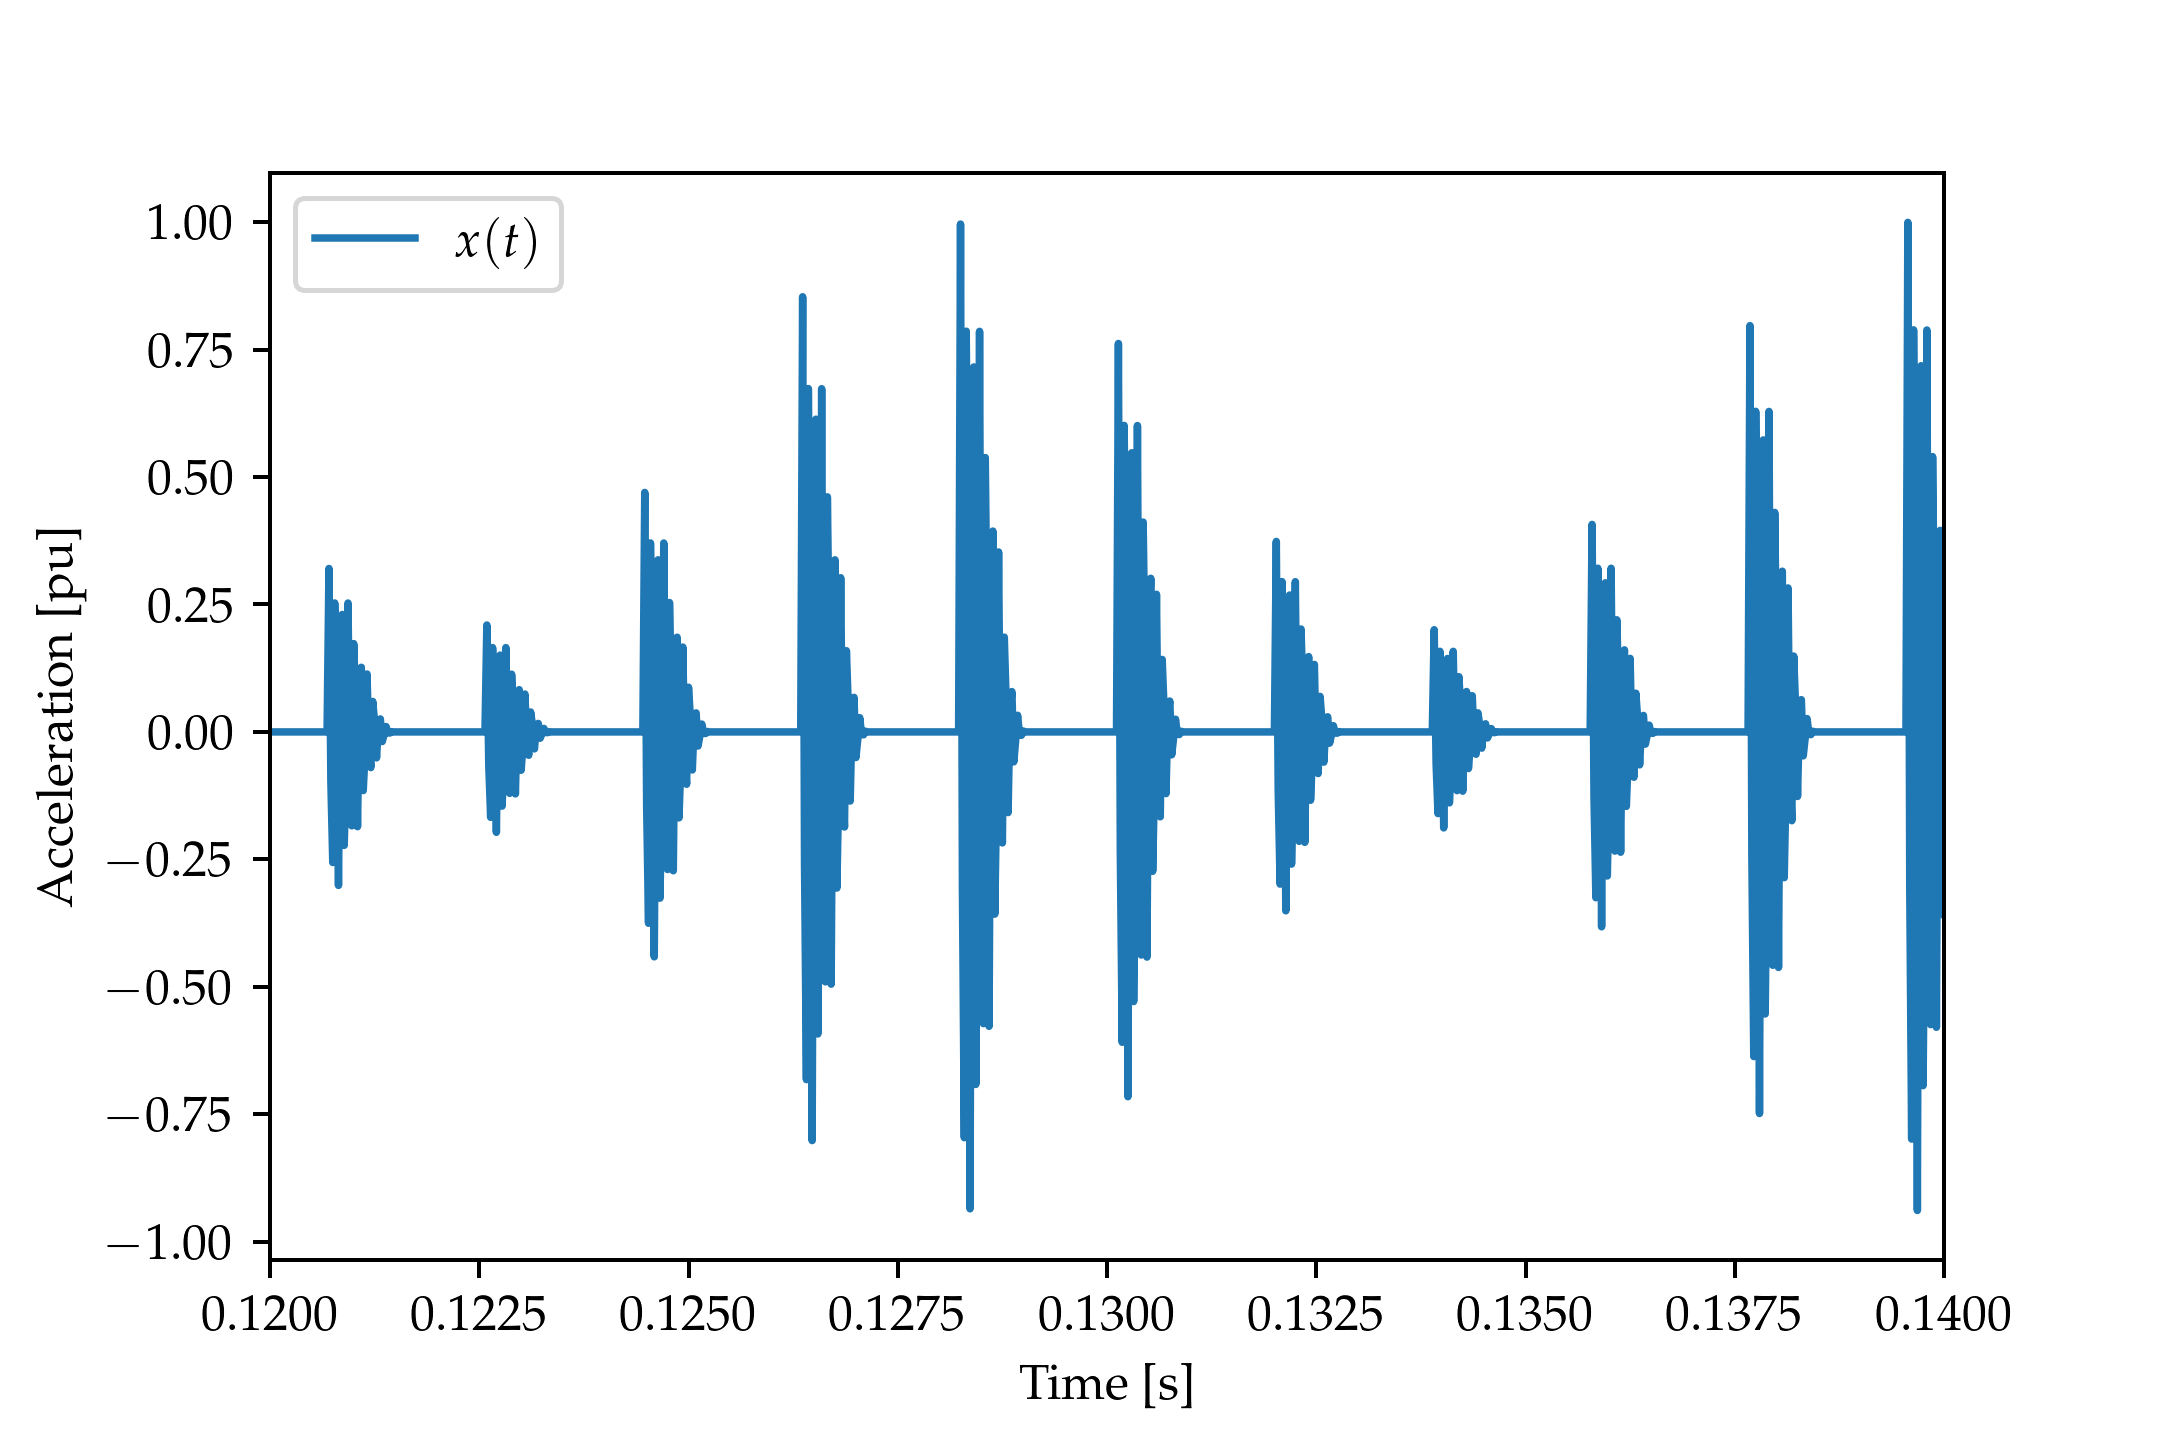
\includegraphics[width=0.5\textwidth]{raw.png}
        \caption{Example of a fingerprint of a damaged roller bearing.}
        \label{fig:raw}
    \end{figure}
    The sampling rate, $f_s$ is usually around $f_s \in [10\text{ kHz}, 100\text{ kHz}]$.
   
\end{frame}